%! Author = Patrik Skaloš
%! login = xskalo01

% Preamble
\documentclass{beamer}

\title{Obojsmerne viazaný zoznam}
\author{Patrik Skaloš}
\date{\today}

% Packages
\usepackage[utf8]{inputenc}
\usepackage[slovak]{babel}
\usepackage{times}
\usepackage{hyperref}
\usepackage{breakurl}
\usepackage{graphicx}
\usepackage[linesnumbered, longend, ruled, czech, noline]{algorithm2e}

\urlstyle{same}
\setbeamertemplate{footline}[frame number]


% Document
\begin{document}
  \frame{\titlepage}

  \begin{frame}
    \frametitle{Úvod}
    \begin{itemize}
      \item Dátové štruktúry programátorom značne uľahčujú prácu.
      \item Je nutné dátové štruktúry poznať a dokázať ich využiť.
      \item Vyhneme sa tým komplikovanej implementácii a strate času
        vynaliezaním niečoho, čo už existuje.
    \end{itemize}
    \bigskip
    V~tejto prezentácii sa zameriam na jednu z~najrozšírenejších dátových 
    štruktúr\,--\,\color{blue}obojsmerne viazaný zoznam.
  \end{frame}

  \begin{frame}
    \frametitle{Obojsmene viazaný zoznam: motivácia}
    \begin{itemize}
      \item Je založený na jednosmerne viazanom zozname, ktorý má veľmi široký 
        záber využitia. Napríklad:
        \begin{itemize}
          \item Vykresľovanie grafov
          \item Imlementácia fronty
          \item Alokácia pamäti
          \item \dots
        \end{itemize}
        \pause
      \item Obojsmerne viazaný zoznam je jednoduchá nadstavba, ktorá:
        \begin{itemize}
          \item Umožňuje pohyb po prvkoch oboma smermi
          \item V mnohých prípadoch aplikáciu zrýchli
          \item Je niekedy dokonca nevyhnutná
        \end{itemize}
        \pause
      \item Používa sa najčastejšie:
        \begin{itemize}
          \item Pri navigácii 
          \item V~internetových prehliadačoch
          \item Vo väčšine aplikácií s možnosťou \textit{undo} a~\textit{redo}
          \item \dots
        \end{itemize}
    \end{itemize}
  \end{frame}
  
  \begin{frame}
    \frametitle{Jednosmerne viazaný zoznam}
    \begin{center}
      \begin{figure}
        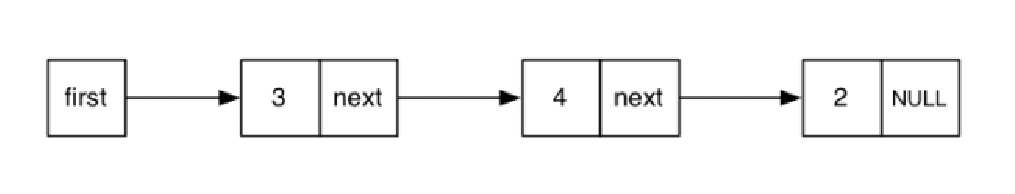
\includegraphics[width=10cm]{./src/sll.eps}
        \caption{Ilustrácia jednosmerne viazaného zoznamu \cite{ll}}
      \end{figure}
    \end{center}
    \begin{itemize}
      \item Na začiatku zoznamu sa nachádza hlava (\textit{anlg. head} alebo 
        \textit{first}), ktorá je ukazovateľom na prvý prvok. 
      \item Posledný prvok nazývame chvost (\textit{angl. tail}). 
      \item Každý z~prvkov okrem dát obsahuje aj ukazovateľ na nasledujúci prvok. 
        \begin{itemize}
          \item V~chvoste je však ukazovateľ na ďalší prvok prázdny.
        \end{itemize}
    \end{itemize}
    \bigskip
    \small Pozn.: Poznáme variáciu \textit{cyklický zoznam}, v~ktorom
    chvost ukazuje na hlavu. Táto variácia je však používaná len zriedka.
  \end{frame}

  \begin{frame}
    \frametitle{Myšlienka obojsmerne viazaného zoznamu}
    \begin{center}
      \begin{figure}
        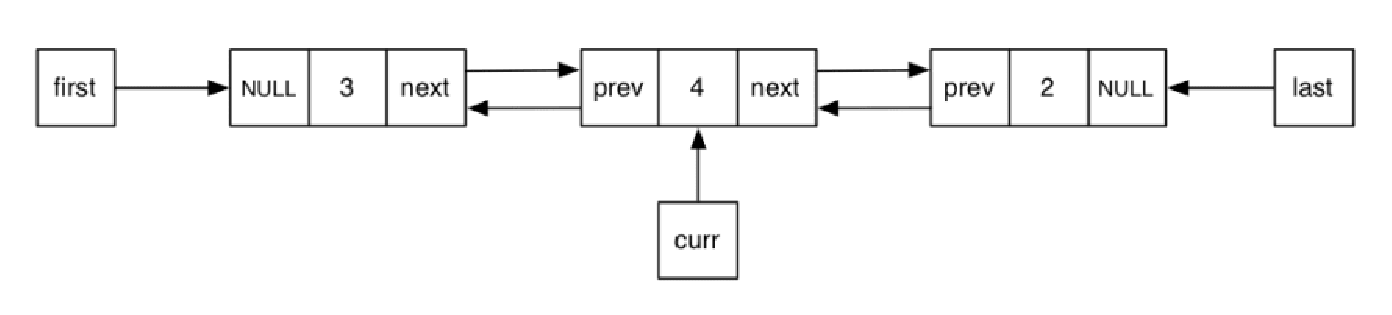
\includegraphics[width=10cm]{./src/dll.eps}
        \caption{Ilustrácia obojsmerne viazaného zoznamu \cite{ll}}
      \end{figure}
    \end{center}
    \begin{itemize}
      \item V každom prvku zoznamu je naviac ďalší ukazovateľ, ktorý je 
        odkazom na predchádzajúci prvok. 
      \item Zoznam sa takto stáva symetrickým.
      \item Niekedy sa pri implementácii používa aj premenná, do ktorej sa ukladá
        ukazovateľ na aktuálnu položku (\textit{angl. current}), ako je to
        zobrazené na obrázku vyššie.
    \end{itemize}
  \end{frame}

  \begin{frame}
    \frametitle{Porovnanie s jednosmerne viazaným zoznamom}
    \textbf{Výhody}
    \begin{itemize}
      \item Možnosť prechádzať zoznam v~oboch smeroch.
      \item Možnosť optimalizácie prehľadávania ak dokážeme v~programe 
        predpokladať, či bude vyhľadávaná položka na začiatku alebo na konci 
        zoznamu.
      \item Efektívnejšie a~rýchlejšie mazanie či vkladanie prvkov vo väčšine 
        prípadoch.
    \end{itemize}
    \pause
    \textbf{Nevýhody}
    \begin{itemize}
      \item Každý prvok obsahuje jeden ukazovateľ naviac.
      \item Pri operáciách so zoznamom treba aktualizovať dvojnásobne viac
        ukazovateľov.
    \end{itemize}
  \end{frame}

  \begin{frame}
    \frametitle{Základné operácie a~ich zložitosť}
    \begin{itemize}
      \item Vyhľadávanie prvku podľa kľúča\,--\,$\mathcal{O}(n)$
      \item Získanie ukazovateľa na hlavu zoznamu\,--\,$\mathcal{O}(1)$
      \item Získanie ukazovateľa na chvost zoznamu\,--\,$\mathcal{O}(1)$
      \item Pridanie prvku do zoznamu\,--\,$\mathcal{O}(1)$
        \begin{itemize}
          \item Na začiatok
          \item Na koniec
          \item Za istý prvok
          \item Pred istý prvok
        \end{itemize}
      \item Vymazanie prvku zo zoznamu\,--\,$\mathcal{O}(1)$
        \begin{itemize}
          \item Prvého prvku
          \item Posledného prvku
          \item Prvku daného ukazovateľom
          \item Prvku daného kľúčom
        \end{itemize}
    \end{itemize}
  \end{frame}

  \begin{frame}
    \frametitle{Pseudokód implementácie mazania prvého prvku zo zoznamu \cite{del}}
    \begin{algorithm}[H]
      \scriptsize
      \label{algo}
      \SetKwInOut{Input}{input}
      \caption{\textsc{Vymazanie prvého prvku}}
      \Input{head, toDelete}
      \If{head points to NULL}{
        return
      }
      \If{toDelete points to NULL}{
        return
      }
      \If{head points to the same node as toDelete}{
        head $\leftarrow$ (toDelete$\rightarrow$next)
      }
      \If{(toDelete$\rightarrow$next) doesn't point to NULL}{
        (toDelete$\rightarrow$next$\rightarrow$prev) $\leftarrow$ (toDelete$\rightarrow$prev)
      }
      \If{(toDelete$\rightarrow$prev) doesn't point to NULL}{
        (toDelete$\rightarrow$prev$\rightarrow$next) $\leftarrow$ (toDelete$\rightarrow$next)
      }
      free the memory pointed to by \textit{toDelete}
    \end{algorithm}
  \end{frame}

  \begin{frame}
    \frametitle{Zdroje}
    \bibliography{proj5}
    \bibliographystyle{czechiso}
  \end{frame}

  \begin{frame}
    \begin{center}
      \vfill
      \huge
      \textbf{Ďakujem za pozornosť} \\
      \vfill
      \large
      Patrik Skaloš
    \end{center}
  \end{frame}

\end{document}
